\section{Governor Model}\label{app:governor_model}
The most important part of a speed governor are the two large masses that rotate on a central axis. These masses are mechanically coupled to the turbine drive shaft, so their angular velocity is a function of the turbine speed. Elgerd and Fosha's text \cite{Elgerd1970} provides a schematic representation of the governing system for a steam turbine, shown in Figure \ref{fig:A01_physical_governor_device}. Borrowing heavily from Kothari \cite{Kothari2011}, this schematic is used to derive the plant model for the governor. 

\begin{figure}[h]
	\centering
	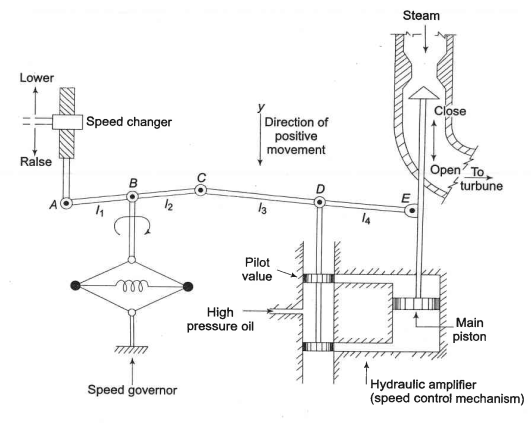
\includegraphics[scale=0.5]{A01_physical_governor_device}
	\caption[Steam governor schematic]{A schematic of a steam governor}
	\label{fig:A01_physical_governor_device}
\end{figure}

Perturbing point $A$ downward some incremental distance, $\Delta y_A$, the turbine power output will change by a directly proportional amount. If $\Delta P_C$ is the power increase, this can be expressed as:
\begin{equation}
	\Delta y_A = k_C \Delta P_C. \label{eq:A01}
\end{equation}

An increase in $\Delta P_C$ will cause the pilot valve to move up, and oil will flow onto the top of the main piston forcing it downwards. As the steam valve opens, more steam will drive the turbine faster causing the governor to lower point $B$. Mathematically, the movement of $C$ can be expressed as the result of two separate inputs:
\begin{enumerate}
	\item Assuming that $\Delta y_A$ is small, using similar triangles, it can be written that:
	\begin{equation}
    	\Delta y_C = - \frac{l_2}{l_1} \Delta y_A.
	\end{equation}
	\item For some frequency increase $\Delta f$, point $B$ will move downward. Assuming $A$ is fixed, by similar triangles it is clear that:
	\begin{equation}
		\Delta y_C = \frac{l_1 + l_2}{l_1} \Delta y_B.
	\end{equation}
\end{enumerate}

Letting $k_1 = \frac{l_2}{l_1}$, $k_2 = \frac{l_1 + l_2}{l_1} k_2'$, and using Equation \ref{eq:A01}, the total movement in point $C$ can be expressed as:
\begin{equation}
	\Delta y_C = - k_1 k_C \Delta P_C + k_2 \Delta f. \label{eq:A02}
\end{equation}

A similar analysis considering perturbation of point $C$ and $E$ can be undertaken to express the movements of point $D$. The analysis makes use of similar triangles and results in the expression:
\begin{equation}
	\Delta y_D = \frac{l_4}{l3 + l_4} \Delta y_C + \frac{l3}{l_3 + l_4} \Delta y_E.
\end{equation}

Letting $k_3 = \frac{l_4}{l_3 + l_4}$ and $k_4 = \frac{l3}{l_3 + l_4}$, this can be re-expressed as:
\begin{equation}
	\Delta y_D = k_3 \Delta y_C + k_4 \Delta y_E. \label{eq:A03}
\end{equation}

Movement, $\Delta y_D$, of point $D$ results in pilot valve ports opening and oil will flowing onto the cylinder causing movement $\Delta y_E$. If point $D$ moves up, oil will force point $E$ down, and conversely if point $D$ moves down, oil will force point $E$ upwards. To simplify the dynamics of this scenario, the following assumptions are made:
\begin{enumerate}
	\item Inertial reaction forces of the main piston and steam valve are negligible compared to the forces exerted on the piston due to the oil
	\item Due to the first assumption, the rate of oil admitted to to the cylinder is proportional to the port opening $\Delta y_D$.
\end{enumerate}

Given the assumptions above, the volume of oil admitted to the cylinder is therefore proportional to the time integral of $\Delta y_D$. Dividing the oil volume by the cross-sectional area of the piston:
\begin{equation}
	\Delta y_E = k_5 \int (- \Delta y_D) dt. \label{eq:A04}
\end{equation}

Taking the Laplace transform of equations \ref{eq:A02}, \ref{eq:A03}, and \ref{eq:A04} yields:
\begin{align}
	\Delta Y_C(s) &= -k_1 k_C \Delta P_C(s) + k_2 \Delta F(s) \label{eq:A05} \\
	\Delta Y_D(s) &= k_3 \Delta Y_C(s) + k_4 \Delta Y_E(s) \label{eq:A06} \\
	\Delta Y_E(s) &= - k_5 \frac{1}{s} \Delta Y_D(s) \label{eq:A07}
\end{align}

Algebraically manipulating \ref{eq:A05}, \ref{eq:A06}, and \ref{eq:A07} eliminates $\Delta Y_C(s)$ and $\Delta Y_D(s)$ and results in the following equation:
\begin{equation}
	\Delta Y_E(s) = \frac{k_1 k_3 k_C \Delta P_C(s) - k_2 k_3 \Delta F(s)}{k_4 + \frac{s}{k_5}}. \label{eq:A08}
\end{equation}

Equation \ref{eq:A08} can be re-expressed as:
\begin{equation}
	\Delta Y_E(s) = \bigg[ \Delta P_C(s) - \frac{1}{R} \Delta F(s) \bigg] \times \bigg( \frac{K_{sg}}{1 + T_{sg}s} \bigg), \label{eq:A09}
\end{equation}

where
\begin{align}
	R &= \frac{k_1 k_C}{k_2} \\
	K_{sg} &= \frac{k_1 k_3 k_C}{k_4} \\
	T_{sg} &= \frac{1}{T_{sg}}.
\end{align}

Equation \ref{eq:A09} is a model of the governor in the frequency domain. The parameter $R$ is referred to as the speed regulation of the governor; the parameter $K_{sg}$ is referred to as the gain of the speed governor; and the parameter $T_{sg}$ is referred to as the time constant of the speed governor.

The complete block diagram of the steam governor model can be seen in Figure \ref{fig:A02_governor_model}.

\begin{figure}[h]
	\centering
	\begin{tikzpicture}

\end{tikzpicture}
	\caption[Steam governor model]{Block diagram of the steam governor model in the frequency domain}
	\label{fig:A02_governor_model}
\end{figure}